% arguelles v2.3.0
% author: Michele Piazzai
% contact: michele.piazzai@uc3m.es
% license: MIT

% Copied from GitHub: https://github.com/piazzai/arguelles

\documentclass[compress,12pt]{beamer}

\usetheme{Arguelles}
\usepackage[german]{babel}
\usepackage{textcomp}
\usepackage[utf-8]{inputenc}
\usepackage[T1]{fontenc}


\title{Bachelorarbeit Visualisierung}
\subtitle{Daten, Fortschritt, erste Ergebnisse, Ideen}
\event{}
\date{}
\author{Christiane Gütter}
\institute{Bauhaus Universität Weimar}

\begin{document}

    \frame[plain]{\titlepage}

    \begin{frame}[plain]
        \frametitle{Themen}
        \begin{enumerate}
            \item Einführung in das Thema
            \item Übersicht grundliegendes Paper
            \item Daten
            \begin{enumerate}
                \item Aufbau
                \item Verarbeitung
            \end{enumerate}
            \item Erste potentielle Fragestellungen
            \item Erste Ergebnisse
            \begin{enumerate}
                \item Erste Visualisierungen
                \item Vergleiche mit Ergebnissen aus Paper
            \end{enumerate}
            \item Nächste Schritte
        \end{enumerate}
    \end{frame}

    \Section{Einfuehrung}

    \begin{frame}[plain,standout]
        \centering
        \textbf{EINFÜHRUNG}
    \end{frame}

    \begin{frame}{r/ChangeMyView}
        \begin{itemize}
            \item Subreddit, i.e.\ ein Forum der großen Social Media Seite Reddit.com
            \item Prinzip:
            \begin{itemize}
                \item OP beschreibt Meinung über ein Thema mit Begründung
                \item Commenters geben (hoffentlich) überzeugende Gegenmeinungen
                \item Vergabe von sog.\ Deltas ($\Delta$\rq{}s) durch OP an überzeugende Gegenargumente
            \end{itemize}
            \item gute Eignung zur Analyse, wegen einfacher \lq\lq{}Messung\rq\rq{} der Überzeugungskraft von Argumenten
        \end{itemize}
    \end{frame}

    \begin{frame}{r/ChangeMyView}
        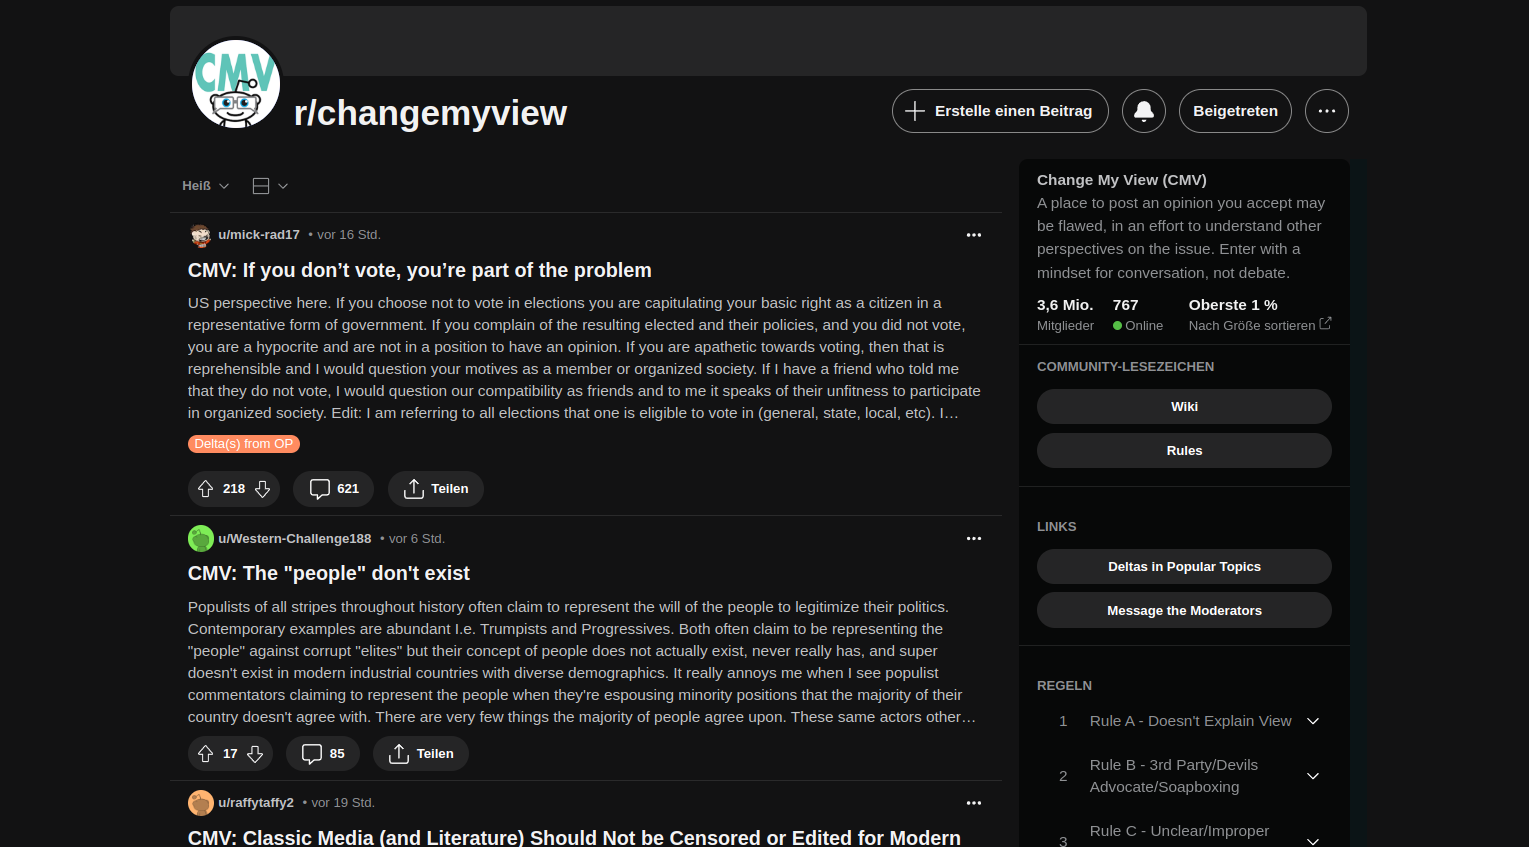
\includegraphics[width=\textwidth]{../images/Screenshot_2024-04-22-15-24-35_1920x1080}
    \end{frame}

    \begin{frame}{r/ChangeMyView}
        \begin{columns}
            \begin{column}{0.5\textwidth}
                
\includegraphics[width=\textwidth]{../images/Screenshot_2024-04-22-15-31-26_1920x1080}
            \end{column}
            \begin{column}{0.5\textwidth}
                
\includegraphics[width=\textwidth]{../images/Screenshot_2024-04-22-15-31-26_1920x1080 (1)}
            \end{column}
        \end{columns}
    \end{frame}

    \begin{frame}{Ziele}
        \begin{itemize}
            \item Unterstützen des Papers der Webis Gruppe durch Visualisierungen
            \item Einsicht geben in Fragen und Problematiken, die das Paper noch offen lässt
            \item Erkenntnisse des Papers mit neuen Fragestellungen erweitern
        \end{itemize}
    \end{frame}

    \End

    \Section{Grundliegendes Paper}

    \begin{frame}[plain,standout]
        \centering
        \textbf{GRUNDLIEGENDES PAPER}
    \end{frame}

    \begin{frame}
        \frametitle{Inhalt}
        {\small
            \begin{quote}
                \lq\lq{}Previous research on argumentation in online discussions has largely focused on \textbf{examining individual comments} and neglected the interactive nature of discussions.
                [\ldots] However, because it is intuitively necessary for dialogical argumentation to address the opposing viewpoints, we extend this model by \textbf{clustering type sequences into different argument arrangement patterns}, thereby \textbf{representing discussions as sequences of these patterns}.
                These sequences of patterns are a \textbf{symbolic representation of argumentation strategies} that capture the overall structure of discussions.[\ldots]\rq\rq{}
            \end{quote}}
    \end{frame}

    \begin{frame}
        \frametitle{Inhalt}
        \begin{itemize}
            \item neuer Ansatz zum Erkennen von argumentativeness
            \item Taggen von Posts und Kommentaren mit sog.\ ADU (argumentative discourse unit) types auf Wortgruppenebene
            \begin{itemize}
                \item \textbf{Value:} \lq\lq{}[\ldots] proposition that refers to subjective value judgments [\ldots]\rq\rq{}
                \item \textbf{Fact:} \lq\lq{}[\ldots] proposition describing objective facts that can be verified using objective evidence [\ldots]\rq\rq{}
                \item \textbf{Policy:} \lq\lq{}[\ldots] a specific course of action to be taken or what should be done [\ldots]\rq\rq{}
                \item \textbf{Testimony:} \lq\lq{}[\ldots]objective proposition related to the author’s personal state or experience [\ldots]\rq\rq{}
                \item \textbf{Rhetorical Statement:} \lq\lq{}[\ldots] subjective value judgment by expressing figurative phrases, emotions, or rhetorical questions [\ldots]\rq\rq{}
            \end{itemize}
        \end{itemize}
    \end{frame}

    \begin{frame}
        \frametitle{Inhalt}
        \begin{itemize}
            \item Zusammenfassen dieser ADU types in Sequenzen auf Kommentarebene
            \item Abstrahieren der Sequenzen
            \item Clustering der Sequenzen in Cluster durch zwei verschiedene Ähnlichkeitsmaße
            \item Nutzen der Sequenzen von Clustern, um persuasiveness mit Transformern zu bestimmen
        \end{itemize}

    \end{frame}

    \begin{frame}
        \frametitle{Inhalt}
        \begin{figure}
            \centering
            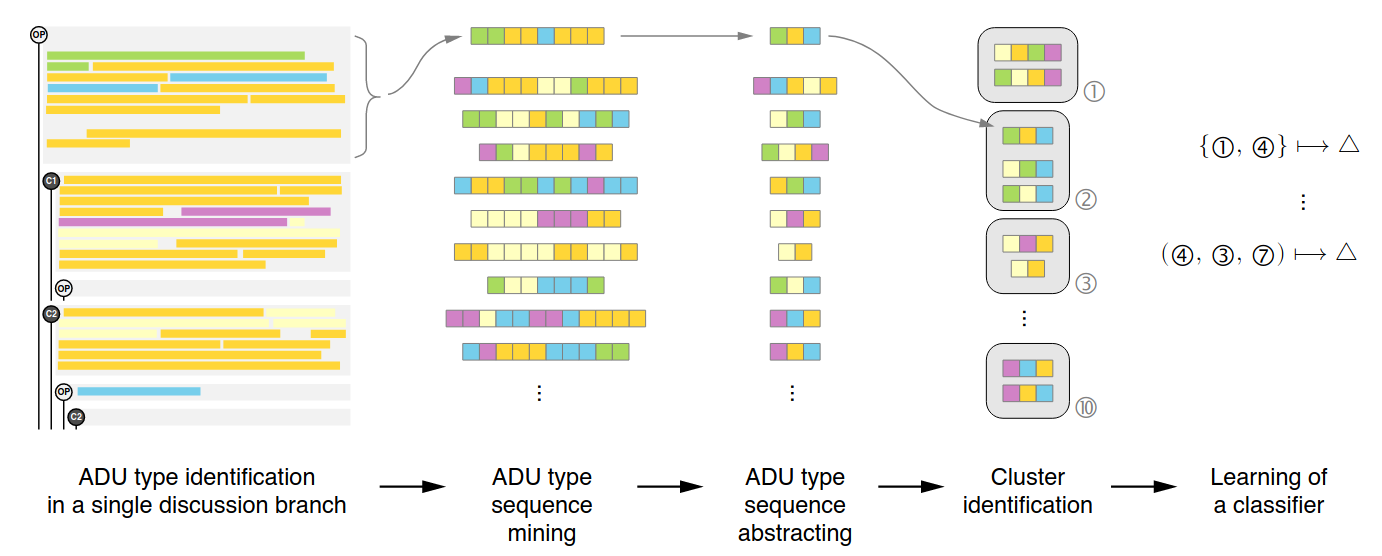
\includegraphics[width=\textwidth]{../images/sequencing}
            \caption{Modeling the overall strategy of two discussion branches as flows of ADU type arrangements per its original post and comments. [...]}
            \label{fig:adu-sequencing}
        \end{figure}
    \end{frame}

    \begin{frame}
        \frametitle{Ergebnisse \& Erkenntnisse}
        \textit{Haupterkenntnis:} Nach Training ist Language Model/Transformer wesentlich besser im Erkennen von stärkeren Argumentationen/Argumentationssträngen als z.B.\ BERT-like Modelle
    \end{frame}

    \begin{frame}
        \frametitle{Ergebnisse \& Erkenntnisse}
        Andere Einsichten:
    \end{frame}

    \begin{frame}{Problematik}
        \begin{itemize}
            \item Abstraktion von Sequenzen und Zusammenfassung in Clustern
            \item Representative Sequenzen der Cluster = die am häufigsten vorkommende Sequenz
            \item einziger Anwendungsfall: persuasion prediction \textrightarrow{} keine Antwort, was eigentlich überzeugend ist
            \item offene Fragen:
            \begin{itemize}
                \item Was ist eigentlich in den Clustern drin?
                \item Sind die representativen Sequenzen aus dem Paper tatsächlich representativ?
                \item Welche Muster gibt es in den Argumentationsstrukturen?
                Kann man als Mensch diese als \lq\lq{}überzeugend\rq\rq{} oder \lq\lq{}nicht überzeugend\rq\rq{} einordnen?
            \end{itemize}
        \end{itemize}
    \end{frame}

    \End

    \Section{Daten}

    \begin{frame}[plain,standout]
        \centering
        \textbf{DATEN}
    \end{frame}

    \begin{frame}{Aufbau}
        \begin{itemize}
            \item Auflistung in JSON Files
            \item einzelnes File = ein Thread/eine einzelne Unterhaltung
            \item Filename = eindeutige ID des OP, Threads aufsteigend nummeriert
            \item Informationen pro Kommentar:
            \begin{itemize}
                \item \texttt{parent\_id}: ID des parent Kommentars (null wenn OP)
                \item \texttt{id}: ID des Kommentar
                \item \texttt{author}: Username des Verfassers
                \item \texttt{title}: Titel des OP (null wenn Kommentar)
                \item \texttt{body}: gesamter OP oder Kommentar
                \item \texttt{preds}: Liste der mit ADU-types getaggten Wortgruppen mit entsprechendem ADU type und certainty score
            \end{itemize}
        \end{itemize}
    \end{frame}

    \begin{frame}{Aufbau}
        \begin{figure}
            \centering
            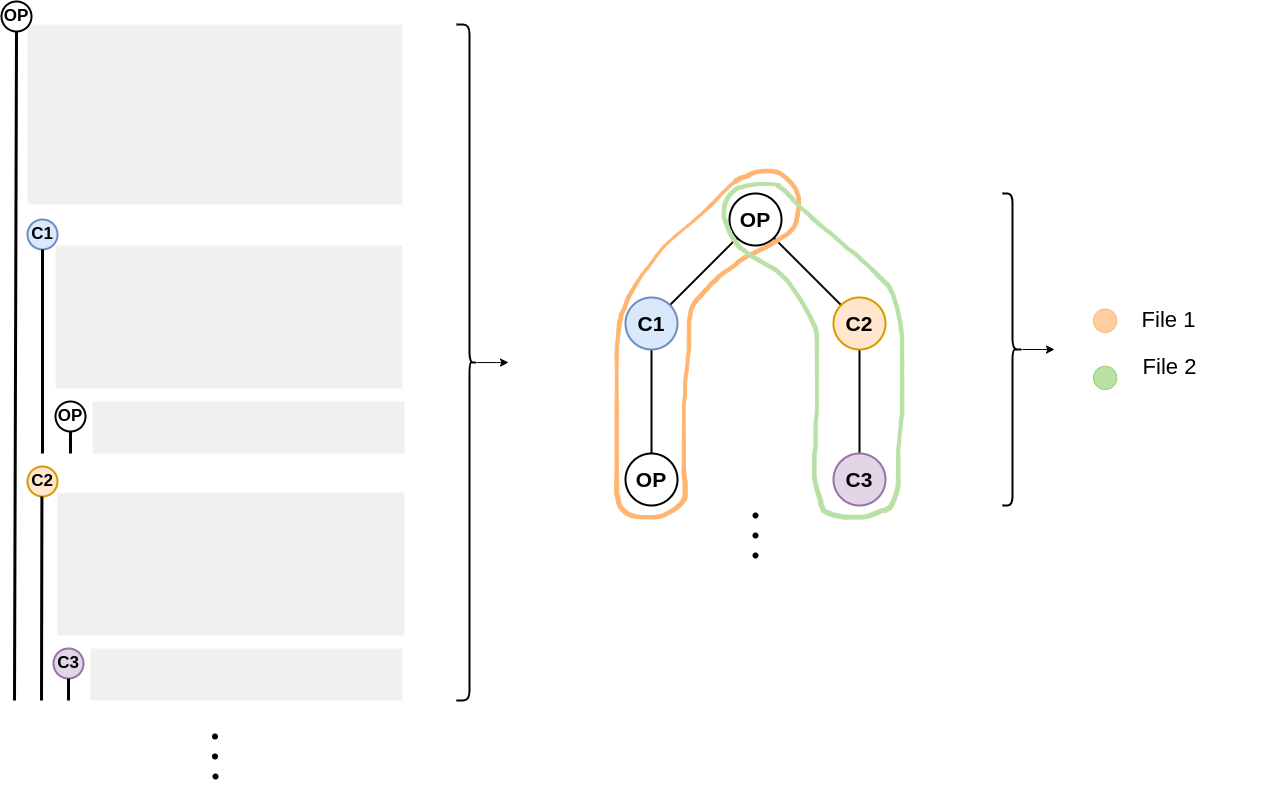
\includegraphics[width=\textwidth]{../images/data-files-structure}
            \caption{Visuelle Aufteilung der Files und deren Inhalt angefangen vom Reddit Post}
            \label{fig:data-structure}
        \end{figure}
    \end{frame}

    \begin{frame}{Aufbau}
        \begin{itemize}
            \item Cluster in eigenen Files
            \item OP Cluster und Comment Cluster getrennt
            \item JSONL Files: eine Zeile = \texttt{[comment\_id, abstract\_adus, sequence, cluster]}
            \begin{itemize}
                \item \texttt{comment\_id}: ID des Kommentar oder Posts
                \item \texttt{abstract\_adus}: Liste mit verkürzter Liste der im Text enthaltenen ADU Types in Worten
                \item \texttt{sequence}: Liste der ADU Types in einzelnen Buchstaben (Anfangsbuchstabe)
                \item \texttt{cluster}: Das Cluster, in welches diese Sequenz eingeordnet wird
            \end{itemize}
        \end{itemize}
    \end{frame}

    \begin{frame}{Verarbeitung}
        \begin{itemize}
            \item per Python Script
            \item Sortieren aller Files mit der gleichen ID (einem Baum angehörig) in einen Unterordner (ID als Name)
            \item Iterieren über alle Unterordner und den enthaltenen Files
            \item Aufbauen eines großen CSV File für das Verarbeiten in d3 mit den nötigen Daten
            \item Verschiedene Eigenschaften werden eingelesen je nach Visualisierung
        \end{itemize}
    \end{frame}

    \End

    \Section{Fragestellungen}

    \begin{frame}[plain,standout]
        \centering
        \textbf{FRAGESTELLUNG}
    \end{frame}

    \begin{frame}{Brainstorming}
        \begin{itemize}
            \item sehr angelehnt an offene Fragestellungen aus dem Paper:
            \begin{itemize}
                \item sinnige Visualisierung vom Inhalt der Cluster
                \item unterstützende Visualisierung um Aufbau der Cluster zu erschließen (representative Eigenschaften)
                \item Strukturen der Threads visuell Untersuchen, um Muster für effektive Argumentationen zu erkennen
            \end{itemize}
        \end{itemize}
    \end{frame}

    \begin{frame}{Brainstorming}
        \begin{itemize}
            \item Untersuchen der User und deren Einfluss:
            \begin{itemize}
                \item in Polylogen: ist Beteiligung von mehr Leuten effektiver?\ Polyloge vs.\ Dialoge?
                \item Sind viele kurze Antworten effektiver als weniger lange?
                \item Bekommen User mit schon vielen Deltas potientiell noch mehr Deltas?
                \item In welchen Clustern kommen welche User vor?
                \item Wie hat die Aktivität von OP die Ergebnisse beeinflusst?\ (Zeit, Menge der Antworten, etc.)
            \end{itemize}
            \item Einfluss des Layouts der Webseite auf die Ergebnisse
        \end{itemize}
    \end{frame}

    \begin{frame}{Ein- und Ausschlüsse}
        \begin{columns}
            \begin{column}{0.5\textwidth}
                \textbf{In Betracht gezogen}
                \begin{itemize}
                    \item Strukturelle Untersuchung der Threads/Bäume
                    \item Visuelle Untersuchung des Inhalts von Clustern
                    \begin{itemize}
                        \item
                    \end{itemize}
                \end{itemize}
            \end{column}
            \begin{column}{0.5\textwidth}
                \textbf{Ausgeschlossen}
            \end{column}
        \end{columns}
    \end{frame}

    \End

    \Section{Erste Visualisierungen}
    \begin{frame}{Threads}

    \end{frame}

    \begin{frame}{Barcharts + Piecharts}

    \end{frame}

    \begin{frame}{Heatmaps + Bars}

    \end{frame}

    \End

    \Section{Erste Ergebnisse}

    \begin{frame}[plain,standout]
        \centering
        \textbf{ERSTE ERGEBNISSE}
    \end{frame}

    \begin{frame}{Unsere Visualisierung}

    \end{frame}

    \begin{frame}{Webis Paper}

    \end{frame}
    \End

    \Section{Naechste Schritte}
    \begin{frame}{Was Lohnt Sich}

    \end{frame}
    \End

    \begin{frame}[plain,standout]
        \centering
        In combination with \textit{plain}, \\
        it makes a nice thank-you slide!
    \end{frame}

\end{document}
